\chapter{Second week}
\section{EDA assignments}
Continuing last week's data exploration, a series of statistical tests were to be read up on and performed.
These tests will be relied upon heavily in the later stages of the project as a form of hypothesis testing.
This analysis aims to explore this subset of the available data and demonstrate sufficient knowledge of statistics and data manipulation.

\subsection{Normality} \label{w2:normality}
All statistical tests described below make certain assumptions about the data they evaluate.
One widespread assumption for a test is that the data will follow a normal distribution.
Since we do not know whether the data is normally distributed, it will be checked using another statistical test.
One such test is the Shapiro-Wilk test.
Of course, these tests come with their own assumptions we'll have to account for.
For Shapiro-Wilk, these assumptions are:
\begin{itemize}
    \item The data is independent.
    \item The dataset contains at least three observations.
    \item The data is continuous.
    \item The data does not contain outliers.
    \item The data is not significantly skewed.
\end{itemize}
While some requirements may be checked off straightaway, others require more work to verify.
Luckily, there are many more normality tests, one of which is Anderson-Darling.
This test is a continuation of the Kolmogorov-Smirnov (K-S) test, allowing us to test for many distributions.
Unfortunately, K-S is less sensitive to deviations in a distribution's tail, an issue that Anderson-Darling solves.

\subsubsection{Methods \& Result}
After loading the dataset into a pandas data frame, the \verb|anderson| function from Scipy's stats package was applied over every column, which equates to every sample.
After transposing the resulting data frame, the following output is produced:

\begin{center}
\begin{tabular}{|l|l|l|l|}
\toprule
 & \bfseries statistic & \bfseries criticalvalues & \bfseries significance \\
\midrule
\bfseries A01\_436578.CEL & 846.411750 & [0.576 0.656 0.787 0.918 1.092] & [15.  10.   5.   2.5  1. ] \\
\bfseries A02\_436580.CEL & 945.752913 & [0.576 0.656 0.787 0.918 1.092] & [15.  10.   5.   2.5  1. ] \\
\bfseries A03\_436582.CEL & 935.441764 & [0.576 0.656 0.787 0.918 1.092] & [15.  10.   5.   2.5  1. ] \\
\bfseries A05\_436586.CEL & 1202.480247 & [0.576 0.656 0.787 0.918 1.092] & [15.  10.   5.   2.5  1. ] \\
\bfseries A06\_436588.CEL & 1036.708589 & [0.576 0.656 0.787 0.918 1.092] & [15.  10.   5.   2.5  1. ] \\
\bfseries A07\_436590.CEL & 1040.810845 & [0.576 0.656 0.787 0.918 1.092] & [15.  10.   5.   2.5  1. ] \\
\bfseries A08\_436610.CEL & 951.268321 & [0.576 0.656 0.787 0.918 1.092] & [15.  10.   5.   2.5  1. ] \\
\bfseries A09\_436608.CEL & 1101.565662 & [0.576 0.656 0.787 0.918 1.092] & [15.  10.   5.   2.5  1. ] \\
\bfseries A10\_436614.CEL & 1119.048689 & [0.576 0.656 0.787 0.918 1.092] & [15.  10.   5.   2.5  1. ] \\
\bfseries A11\_436612.CEL & 901.104212 & [0.576 0.656 0.787 0.918 1.092] & [15.  10.   5.   2.5  1. ] \\
\bottomrule
\end{tabular}

\end{center}

\par We may then select a critical value based on the significance level we want to use.
If the statistic is higher than the corresponding critical value, we may conclude that the data does not conform to the chosen distribution.
Doing this for all 1067 samples, we find that none are normally distributed ($\alpha = 0.05$).

\subsection{ANOVA}

\subsubsection{Use}
The one-way ANOVA is used to compare the means of three or more independent groups from differing populations.

\subsubsection{Assumptions}
\begin{itemize}
    \item Groups are independent of one another.
    \item The data is normally distributed.
    \item There exists a similar amount of variance within groups.
\end{itemize}

\subsubsection{Adherence to assumptions}
\paragraph{Independence}
Each column represents a sample, which presumably is independent of other samples.
This has, however, not been checked.

\paragraph{Normality}
As discussed in \ref{w2:normality}, none of the samples are normally distributed.
Therefore, the data does not adhere to this assumption

\paragraph{Variance}
This has not been checked since, thus far, this has been a demonstration.
However, this might be worth investigating when exploring the full dataset.

\subsubsection{Methods \& Results}
Despite the lack of adherence to all of ANOVA's assumptions, the test was performed regardless as a proof of concept.
Every sample was passed to ANOVA as a group, therefore testing whether the mean of each sample is, statistically speaking, equal.
This produced the following results:
\begin{itemize}
    \item $F = 11.963$
    \item $p = 0.0$
\end{itemize}

Since $p < 0.05$, we may reject the $H_0$ hypothesis and conclude that the means of each sample are not equal.

\subsection{Kruskal-Wallis test}

\subsubsection{Use}
To compare the means of three or more independent groups from differing populations.
This test is the non-parametric equivalent of ANOVA.
It does not assume normality and is less sensitive to outliers.

\subsubsection{Assumptions}
\begin{itemize}
    \item Response variable should be ordinal or continuous.
    \item Groups are independent of one another.
    \item Distributions within each group have similar shapes.
\end{itemize}

\subsubsection{Adherence to assumptions}
\paragraph{Ordinal or continuous}
We are working with a continuous series of expression levels.
Therefore, the data adheres to this assumption.

\paragraph{Independence}
Each column represents a sample, which presumably is independent of other samples.
This has, however, not been checked.

\paragraph{Distribution shapes}
This has not been checked since, thus far, this has been a demonstration.
However, this might be worth investigating when exploring the full dataset.

\subsubsection{Methods \& Results}
Although not all of Kruskal-Wallis' assumptions were accounted for, the test was performed regardless as a proof of concept.
Every sample was passed to the test as a group, therefore testing whether the median of each sample is, statistically speaking, equal.
This produced the following results:
\begin{itemize}
    \item $F = 13723.614$
    \item $p = 0.0$
\end{itemize}

Since $p < 0.05$, we may reject the $H_0$ hypothesis and conclude that the medians of each sample are not equal.

\subsection{T-Test}
A t-test is a statistical test used to compare the means of two groups or the mean of a group to a standard value.
A range of differing t-tests exist, all with their distinct purpose.
A selection of the most commonly used t-tests was considered before choosing the Welch t-test for this comparison.

\subsubsection{Use}
To compare the means of two independent groups from differing populations.

\subsubsection{Assumptions}
Most t-tests, including the one-sample, two-sample, and paired t-tests, make the following assumptions about the data that is to be tested:
\begin{itemize}
    \item Groups are independent of each other.
    \item Data follows a normal distribution.
    \item The variance within each group is similar.
\end{itemize}

\subsubsection{Adherence to assumptions}
\paragraph{Independence}
Each column represents a sample, which presumably is independent of other samples.
This has, however, not been checked.

\paragraph{Normality}
As discussed in \ref{w2:normality}, none of the samples are normally distributed.
Therefore, the data does not adhere to this assumption

\paragraph{Variance}
Most t-tests require the variance within each group to be similar.
Statistical methods exist to ensure the data adheres to this assumption, but another solution exists.
The Welch t-test was specifically chosen for its indifference to the amount of variance within groups.
In datasets where variance is not an issue, Welch may still be used as it performs as well as a regular two-sample t-test.

\subsubsection{Result}
Every sample in the dataset was compared to every other sample using a Welch t-test.
Since the dataset consists of over one thousand samples, this produced over one million p-values.
To visualise this many values, a heatmap was made.

\begin{figure}[H]
    \centering
    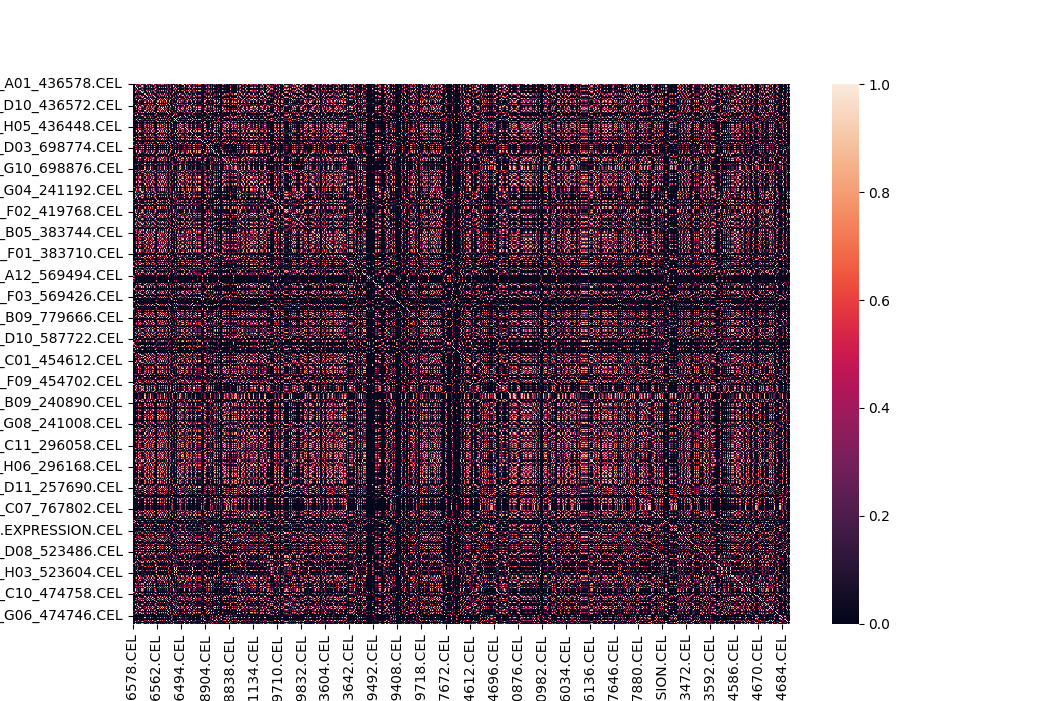
\includegraphics[scale=0.6]{pvalues_samples_ttest}
    \caption{Heatmap showcasing p-values for each sample comparison made using Welch t-tests}
    \label{plt:ttesthm}
\end{figure}

As seen in figure \ref{plt:ttesthm}, there exist black horizontal lines where p-values are near zero.
The Welch t-test's $H_0$ hypothesis states that population means are equal.
Since p-values in these dark bands are very low, this indicates that, in these regions, the $H_0$ hypothesis may be rejected.
Therefore, a lot of variability exists in these specific regions.
\par A diagonal white line is visible in the figure.
This represents a sample being compared with itself, therefore producing a p-values of one since these groups are identical.

\subsection{Mann-Whitney U}

\subsubsection{Use}
The Mann-Whitney U test serves as a non-parametric equivalent of the two-sample t-test.
While the two are equal in many respects, the Mann-Whitney U test does not assume normality and is meant for smaller sample sizes (n < 30).

\subsubsection{Assumptions}
\begin{itemize}
    \item Response variable should be ordinal or continuous.
    \item Groups are independent of one another.
    \item Distributions within each group have similar shapes.
\end{itemize}

\subsubsection{Adherence to assumptions}
\paragraph{Ordinal or continuous}
We are working with a continuous series of expression levels.
Therefore, the data adheres to this assumption.

\paragraph{Independence}
Each column represents a sample, which presumably is independent of other samples.
This has, however, not been checked.

\paragraph{Distribution shapes}
This has not been checked since, thus far, this has been a demonstration.
However, this might be worth investigating when exploring the full dataset.

\subsubsection{Result}
Every sample in the dataset was compared to every other sample using a Mann-Whitney U test.
Since the dataset consists of over one thousand samples, this produced over one million p-values.
To visualise this many values, a heatmap was made.

\begin{figure}[H]
    \centering
    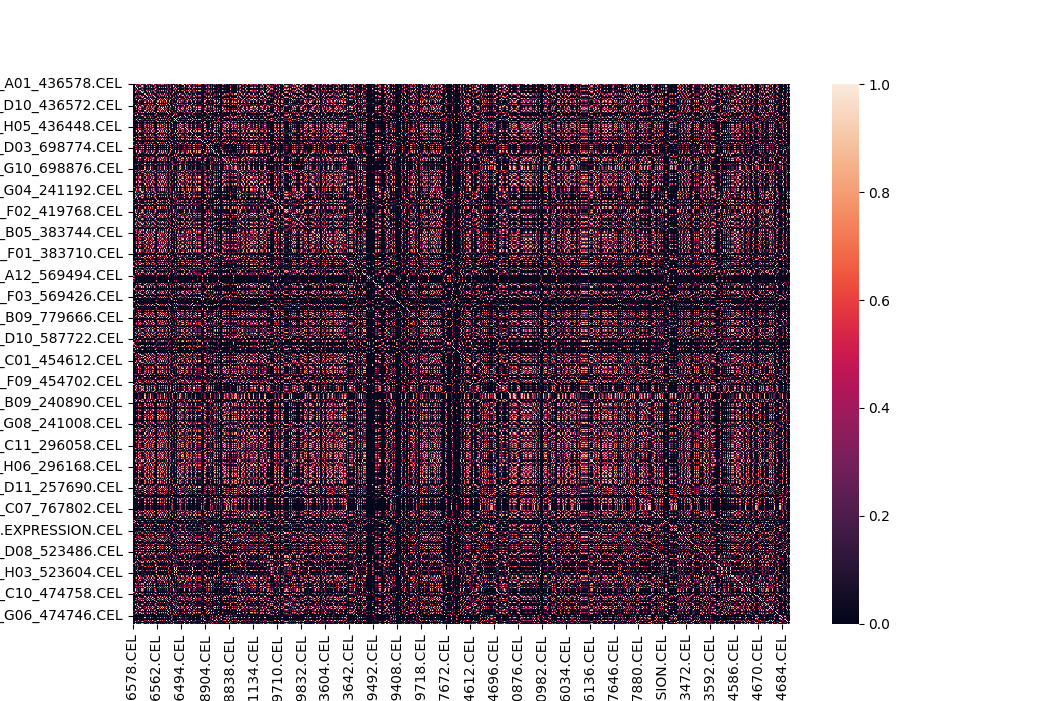
\includegraphics[scale=0.6]{pvalues_samples_mannwhitneyu}
    \caption{Heatmap showcasing p-values for each sample comparison made using Mann-Whitney U tests}
    \label{plt:mwuhm}
\end{figure}

As seen in figure \ref{plt:mwuhm}, there exist black horizontal lines where p-values are near zero.
The Mann-Whitney U test's $H_0$ hypothesis states that population means are equal.
Since p-values in these dark bands are very low, this indicates that, in these regions, the $H_0$ hypothesis may be rejected.
Therefore, a lot of variability exists in these specific regions.

A diagonal white line is visible in the figure.
This represents a sample being compared with itself, therefore producing a p-values of one, since these groups are identical.

Note that figure \ref{plt:mwuhm} is identical to \ref{plt:ttesthm}, although the former was produced with the Welch t-test and the latter with the Mann-Whitney U test.

\subsection{Fisher's Exact}

\subsubsection{Use}
Fisher's exact test is used to check if two categorical variables are significantly associated.
This test serves as an alternative to the Chi-Square test when sample sizes are small ($n \le 5$ per cell or $cell counts \le 20$).

\subsubsection{Assumptions}
\begin{itemize}
    \item Groups are independent of one another.
    \item The variable of interest is proportional or categorical.
    \item Groups are mutually exclusive.
\end{itemize}

\subsubsection{Adherence to assumptions}
\paragraph{Independence}
Each row represents a gene, which presumably is mostly independent of other genes.
This has, however, not been checked.

\paragraph{Proportional or categorical}
The dataset at hand does not inherently lend itself to categorical analysis.
Nevertheless, we'll want to perform this test for demonstration purposes.
We will therefore have to make up our own categories.

\paragraph{Mutual exclusivity}
Genes are mutually exclusive.
As discussed above, the second categorical variable to perform the test on will have to be artificial.
Since we are in control, we can make sure it is mutually exclusive.

\subsubsection{Methods \& Results}
To perform this test, two genes were chosen at random as the first categorical variable.
To create a second categorical variable, the expression levels for these genes were separated into two groups:
Those with expression levels above 3.5, and those with expression levels below.
The 3.5 cutoff point was chosen arbitrarily.
This produced the following results:

\begin{center}
\begin{tabular}{|l|l|l|l|}
\toprule
 & \bfseries 1560957\_at & \bfseries 205483\_s\_at \\
\midrule
\bfseries > 3.5 & 615 & 1066 \\
\bfseries < 3.5 & 452 & 1 \\
\bottomrule
\end{tabular}

\end{center}

\begin{itemize}
    \item $Statistic = 0.00127$
    \item $p = 1.147e^{-160}$
\end{itemize}

Since $p < 0.05$, we may reject the $H_0$ hypothesis and conclude that the two variables are not significantly associated.

\section{Action plan}
Did not get much of anything done this week.

\section{Project Logbook}
Yes, the very document you are reading right now!
Scattered notes, code, and a few folders with plots aren't the best way to keep track of what you are doing and what you have found.
So, that's where this document comes in.
A week-by-week log of what I've been up to.

I keep this document informative with the knowledge I have gathered, analyses I've run, and conclusions.
However, I will not be overly formal, especially while I am still figuring things out.

\section{GitHub}
With a small collection of scripts and text documents coalescing, I am considering creating a GitHub repository to keep track of it all.
As of now, all work exists on my local machine and a cloud backup, but there is no version control in place.
I am still considering whether this current exploration phase should be within the same repository as the eventual product will be.
A central repository containing all relevant materials (product code, EDA code, logbook, report, poster, etc.) does seem reasonable, but it is something I should probably decide on in consultation with my supervisor.

I did create a GitHub project this week as way of tracking to-dos.
Once a repository is in place, this project may be associated with the repository.
I may then make use of GitHub issues in my to-dos and assign them to milestones to keep track of the timeline.
